\chapter{Vehicle Model}

We need to be able to simulate the motion of the vehicle during the process of trajectory planning. If we would know the exact state of the vehicle after performing each action starting in the initial state, we could determine whether the plan keeps the vehicle on the track, avoids all of the obstacles, and what the time for reaching the goal state is. This would enable us to pick a safe time-optimal plan for the racing car.

\section{Problem Definition}

\paragraph{Vehicle model} is a function $v: S \times A \rightarrow S$, where $S$ is the state space and $A$ is the action space, which for a given state $s = ( \, \vec{0}, \vec{v}, \alpha, \theta ) \, \in S$ and an action $a = ( \, t, \phi ) \, \in A$ predicts a new state $s\prime$ in which the vehicle will most likely be after performing the action $a$ for a time period of $t_{const}$ seconds.

We assume that the position of the vehicle is the origin of the vector space because we are interested only in the change of position and we can easily calculate the new absolute position of the vehicle by adding the old position with the position change.

Given the non-deterministic nature of the real world and the hardware limitations of the vehicle we can never assume that our prediction will be correct. Our model of the world is considerably simple and does not take into account many aspects of the real world such as weather, road material, or vehicle depreciation (e.g., the wear of tires or breaks, mechanical issues). 

% todo: how to fight this problem? probabilities? what about cumulation of error?

\section{The Kinematic Bicycle Model}

One of the simplest vehicle models used for trajectory planning is the kinematic bicycle model \cite{bicycleModel}. In this model we merge the two front wheels (resp. the two rear wheel) into a single wheel located at the center of the axle. The control inputs then consists of acceleration \(t\) and the front wheel steering angle \(\phi\). The schema of this model can be seen in figure ~\ref{fig:bicycleModel}.

We can describe the model using these equations:

\begin{align*}
    x' &= |\vec{v}|\cos\big(\psi + \beta(\phi)\big) \\
    y' &= |\vec{v}|\sin\big(\psi + \beta(\phi)\big) \\
    v' &= t \\
    \psi &= \frac{|\vec{v}|}{l_r}\sin\big(\beta(\phi)\big),
\end{align*}

where \(\beta(\phi)\) is the slip angle at the center of gravity:

\[
    \beta (\phi) = \arctan\Big(\tan(\psi)\frac{l_r}{l_f + l_r}\Big).
\]

\begin{figure}
    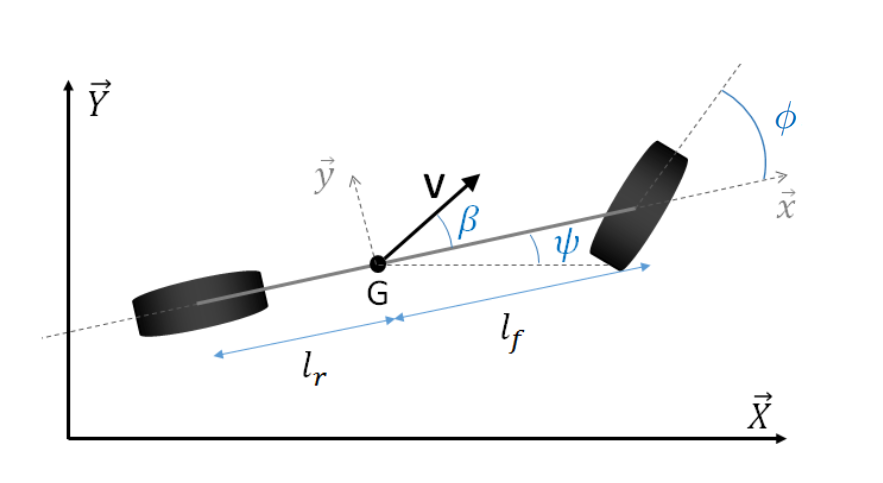
\includegraphics[width=\textwidth]{../img/bicycle-model.png}
    \centering
    \caption{The kinematic vehicle model schema \cite{bicycleModel}}
    \label{fig:bicycleModel}
\end{figure}

\section{Machine Learning}

Another approach we could use is to use machine learning. We could collect enough data from the sensors while driving the vehicle manually and match the actions with the measured state of the vehicle. With enough data, it should be possible to train a model which would predict the change of the vehicle state.

A downside of this approach is that with each change of the vehicle parameters (e.g., different motor, change of weight of the vehicle, different surface of the racing track) we would need to collect the whole data set and train the model again. This is not a problem for us as we want to perform experiments only on a single type of a vehicle.

An upside of the machine learning model can be that with enough data, the model can learn to consider the dynamics of the vehicle which are hard to describe with equations or which would be computationally expensive (e.g., drifting, the slip angle) \cite{}.

\subsection{Training Data}

We can collect data by driving the vehicle on a test track while collecting the data from its sensors. This gives us two streams of data: a stream of actions we used to control the vehicle and a stream of vehicle states which was calculated based on the data from the sensors. All of these data will contain timestamps, but will be most definitely emitted with different frequencies and out of sync. The actions must be sent at a constant time period $t_{const}$. The frequency of the vehicle states depends directly on the capabilities of the sensors, most notably the rotation speed of the LIDAR. We can assume that the frequency at which we collect the data from the controller is higher than the frequency at which we collect vehicle states.

The training data should contain all possible actions and all possible vehicle states in terms of velocity and orientation as the vehicle model does not consider the absolute position of the vehicle when the action is performed.

\subsection{Reinforcement Learning}

It would be hard to use supervised learning to train a model using our data set. We do not know the state of the vehicle at the time when we perform some action with the exception of the initial state and the first action and we would not know the exact state at the and of performing the given action because the next state might be measured with a considerable delay.

A better approach in our scenario would be to use reinforcement learning (RL). We would start in the initial state and use our model to predict several consecutive states after applying several actions. We would then give the model a reward based on how close this predicted states were to the observed states and whether the model predicted the goal state accurately.

\paragraph{NeuroEvolution of Augmenting Topologies} (NEAT) is an reinforcement learning algorithm based published by Kenneth O. Stanley and Risto Miikkulainen. It is an artificial evolution of neural network using genetic algorithms \cite{neat}. (todo: write more about NEAT)

\paragraph{Q-learning} (todo: describe the basics of Q-learning)

% todo describe some RL algos and why we would use NEAT

\section{Evolution of the Dynamic Model}

\subsection{Evolution Setup}

\subsection{The Reward Function}

\subsection{Results}